\documentclass[12pt,class=report,crop=false]{standalone}
\usepackage[screen]{../python}


\pagestyle{empty}

\begin{document}

% Commande spécifique
\newcommand{\badletter}[1]{\underline{\textcolor{red}{#1}}}



%====================================================================
\chapitre{Images dynamiques}
%====================================================================


\section*{Transformation du photomaton}


On part d'un tableau $n\times n$, avec $n$ pair, chaque élément du tableau représente un pixel. 

\myfigure{0.7}{
\tikzinput{fig-images-1}
}


\medskip
\mybox{
Pour chaque couple $(i,j)$, on calcule son image $(i',j')$ par la transformation du photomaton selon les formules suivantes :
\begin{itemize}
  \item Si $i$ et $j$ sont pairs : $(i',j') = (i//2,j//2)$.
  \item Si $i$ est pair et $j$ est impair : $(i',j') = (i//2,(n+j)//2)$.  
  \item Si $i$ est impair et $j$ est pair : $(i',j') = ((n+i)//2,j//2)$.
  \item Si $i$ et $j$ sont impairs : $(i',j') = ((n+i)//2,(n+j)//2)$.
\end{itemize}
}
\newpage

\medskip
\emph{Exemple.} 

$$\begin{array}{cccc} 
  1& 2& 3& 4\\ 
  5& 6& 7& 8\\  
  9&10&11&12\\  
 13&14&15&16  
\end{array}\qquad\qquad  
\begin{array}{cccc} 
  1& 3& 2& 4\\  
  9&11&10&12\\  
  5& 7& 6& 8\\  
 13&15&14&16
\end{array}$$


\newpage

Voici une image $256 \times 256$ et sa première transformation :

\begin{center}
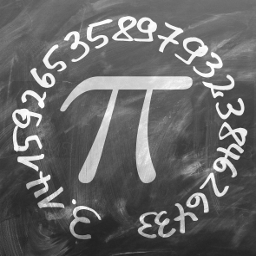
\includegraphics[scale=0.4]{images_fiche/pi_gimp_new_photo_0.png}\qquad\qquad
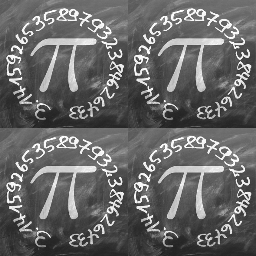
\includegraphics[scale=0.4]{images_fiche/pi_gimp_new_photo_1.png}
\end{center}

Voici ce qui se passe si on répète plusieurs fois la transformation du photomaton :
\begin{center}

\includegraphics[scale=0.3]{images_fiche/pi_gimp_new_photo_2.png}\qquad

\includegraphics[scale=0.3]{images_fiche/pi_gimp_new_photo_3.png}\qquad
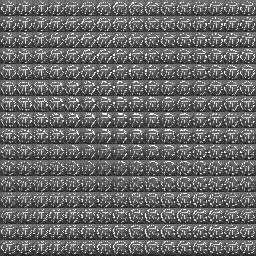
\includegraphics[scale=0.3]{images_fiche/pi_gimp_new_photo_4.png}
\end{center}
\begin{center}
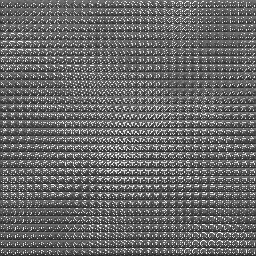
\includegraphics[scale=0.3]{images_fiche/pi_gimp_new_photo_5.png}\qquad
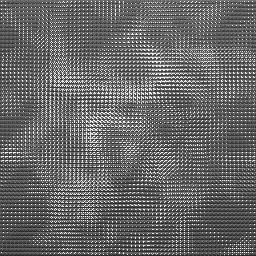
\includegraphics[scale=0.3]{images_fiche/pi_gimp_new_photo_6.png}\qquad
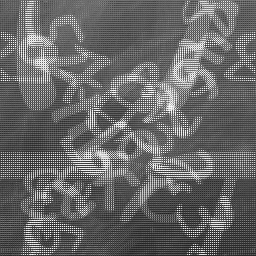
\includegraphics[scale=0.3]{images_fiche/pi_gimp_new_photo_7.png}\qquad
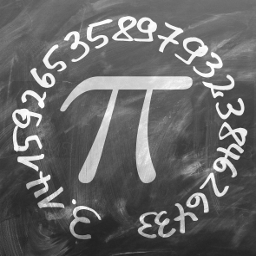
\includegraphics[scale=0.3]{images_fiche/pi_gimp_new_photo_8.png}
\end{center}

\newpage

Tu peux initialiser un nouveau tableau par la commande :\\
  \centerline{\ci{nouv_tableau = [[0 for j in range(n)] for i in range(n)]}}
  
 Puis le remplir par des commandes du type :\\
  \centerline{\ci{nouv_tableau[ii][jj] = tableau[i][j]}}


\newpage

\evidence{Format \og{}pgm\fg{}}

Fichier image au format \og{}pgm\fg{} à partir d'un tableau de niveaux de gris.
  
\begin{center}
\begin{minipage}{0.3\textwidth}
\begin{lstlisting}
P2
5 5
255
128 192 128 192 128
224   0 228   0 224
228 228 228 228 228 
224  64  64  64 224 
192 192 192 192 192 
\end{lstlisting}
\end{minipage}
\begin{minipage}{0.3\textwidth}
\begin{center}

\includegraphics[scale=0.15]{input/ecran-test-pgm}
\end{center}
\end{minipage}
\end{center}
  
 
 
\newpage

 
 
\section*{Transformation du boulanger}

On part d'un tableau $n\times n$, avec $n$ pair dont chaque élément représente un pixel. 
On va appliquer deux transformations élémentaires à chaque fois.

\evidence{Étirer.} Le principe est le suivant : les deux premières lignes (chacune de longueur $n$) produisent une seule ligne de longueur $2n$ en mixant les valeurs de chaque ligne en alternant un élément du haut, un élément du bas.

\medskip
 
\myfigure{1}{
\tikzinput{fig-images-2}
}


\myfigure{1}{
\tikzinput{fig-images-2bis}
}  

\medskip

\mybox{
\emph{Formules.} Un élément en position $(i,j)$ du tableau d'arrivée, correspond à un élément $(2i,j//2)$ (si $j$ est pair) ou bien $(2i+1,j//2)$ (si $j$ est impair) avec ici $0 \le i < \frac n2$ et $0 \le j < 2n$.
}

\newpage


\emph{Exemple.} Voici un tableau $4 \times 4$ à gauche, et le tableau étiré $2 \times 8$ à droite.
Les lignes $0$ et $1$ à gauche donnent la ligne $0$ à droite.
Les lignes $2$ et $3$ à gauche donne la ligne $1$ à droite.
$$\begin{array}{cccc} 
  1& 2& 3& 4\\ 
  5& 6& 7& 8\\  
  9&10&11&12\\  
 13&14&15&16  
\end{array}\qquad\qquad 
\begin{array}{cccccccc} 
  1& 5& 2& 6& 3& 7& 4& 8  \\
  9&13&10&14&11&15&12&16
\end{array}$$
  
 \newpage 
  
\evidence{Replier.} Le principe est le suivant : la partie droite d'un tableau étiré est retournée, puis ajoutée sous la partie gauche. Partant d'un tableau $\frac n2 \times 2n$ on obtient un tableau $n \times n$.

 
\myfigure{0.7}{
\tikzinput{fig-images-3}
}  

\mybox{
\emph{Formules.} 
Pour $0 \le i < \frac n2$ et $0 \le j < n$ les éléments en position $(i,j)$ du tableau sont conservés.
Pour $\frac n2 \le i < n$ et $0 \le j < n$ un élément du tableau 
d'arrivée $(i,j)$, correspond à un élément $\big(\frac{n}{2} - i - 1,2n-1-j\big)$ du tableau de départ. 
}

\newpage


\emph{Exemple.} 
À partir du tableau étiré $2 \times 8$ à gauche, on obtient un tableau replié $4 \times 4$ à droite. 
$$ 
\begin{array}{cccccccc} 
  1& 5& 2& 6& 3& 7& 4& 8  \\
  9&13&10&14&11&15&12&16
\end{array}\qquad\qquad
\begin{array}{cccc} 
  1& 5& 2& 6\\ 
  9& 13& 10& 14\\  
  16&12&15&11\\  
  8&4&7&3  
\end{array}$$


\newpage


La \defi{transformation du boulanger} est la succession d'un étirement et d'un repliement. Partant d'un tableau $n \times n$ on obtient encore un tableau $n \times n$.


Voyons un exemple de l'action de plusieurs transformations du boulanger.
À gauche l'image initiale de taille $128 \times 128$, puis le résultat de $k=1,2,3$ itérations. 
\begin{center}

\includegraphics[scale=0.6]{images_fiche/surf_gimp_new_boul_0.png}\qquad
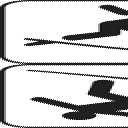
\includegraphics[scale=0.6]{images_fiche/surf_gimp_new_boul_1.png}\qquad

\includegraphics[scale=0.6]{images_fiche/surf_gimp_new_boul_2.png}\qquad
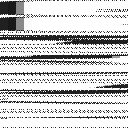
\includegraphics[scale=0.6]{images_fiche/surf_gimp_new_boul_3.png}
\end{center}


Voici les images pour $k=12,13,14,15$ itérations :
\begin{center}
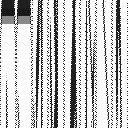
\includegraphics[scale=0.6]{images_fiche/surf_gimp_new_boul_12.png}\qquad
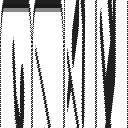
\includegraphics[scale=0.6]{images_fiche/surf_gimp_new_boul_13.png}\qquad
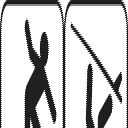
\includegraphics[scale=0.6]{images_fiche/surf_gimp_new_boul_14.png}\qquad

\includegraphics[scale=0.6]{images_fiche/surf_gimp_new_boul_15.png}
\end{center}


\end{document}
